\section{Experiments}\label{sec:exp}
We demonstrate the effectiveness and efficiency of our Sliceformer through comprehensive comparative and analytic experiments. 
In particular, we first compare our Sliceformer to Transformer and its representative variants on the Long Range Arena benchmark~\cite{tay2021long} and empirically verify the rationality of our slicing-sorting operation. 
Then, we implement ViT~\cite{dosovitskiy2021an} by our Sliceformer and test its performance and permutation-invariance in image classification tasks. 
Finally, we impose our slice-sorting operation on Graphormer~\cite{ying2021transformers}, leading to a Sliceformer for graph-structured data. 
This model achieves comparable performance in molecular representation with fewer parameters, demonstrating the universal applicability of our slice-sorting attention layer.
\textbf{Representative results are shown below. More results and implementation details are in the supplementary file. 
}


\subsection{Long Range Arena Benchmark}
Long Range Arena (LRA) is a benchmark designed to evaluate models for long sequence scenarios~\cite{tay2021long}, which consists of six discriminative learning tasks, including ListOps~\cite{nangia2018listops}, byte-level text classification~\cite{maas2011learning}, byte-level document retrieval~\cite{radev2013acl}, and three image classification tasks on CIFAR-10~\cite{krizhevsky2009learning}, Pathfinder~\cite{linsley2018learning},\footnote{Pathfinder is an image classification task: given a set of gray-level images, each of which plots two points and several curves, the model aims to recognize whether there exists a path connecting the points in each image.} and Pathfinder-X (a longer and more challenging version of Pathfinder). 
In the three image classification tasks, each image is formulated as a sequence of pixels.
We test our Sliceformer on the LRA benchmark and compare it to other Transformer-based models on both prediction accuracy and computational efficiency. 
In each task, our Sliceformer is trained to represent each input sequence through the embedding in the ``CLS'' position. 
For a fair comparison, we implement all the models based on JAX~\cite{bradbury2018jax} and strictly follow the benchmark's default data processing and experimental design.
In each task, our Sliceformer is the same as the other models on the number of layers and the dimension of hidden variables. 
Hence, its model parameters are fewer because of abandoning the ``query-key-value'' attention architecture. 
All the models are trained on 4 NVIDIA 3090 GPUs. 




\begin{table}[t]
  \centering
  \caption{The comparison for various models on the LRA benchmark. 
  ``FAIL'' means the training process fails to converge.
  In each column, we bold the best result and underline the second best one.}
  \small{
    \begin{tabular}{l|cccccc|c}
    \toprule
    \multicolumn{1}{c|}{Model} & ListOps & Text  & Retrieval & Image & Path  & Path-X & Avg. Acc (\%)\\
    \midrule
    Transformer~\cite{vaswani2017attention} & 36.37 & 64.27 & 57.46 & 42.44 & 71.40 & FAIL  & 54.39 \\
    \midrule
    Local Attention~\cite{tay2021long} & 15.82 & 52.98 & 53.39 & 41.46 & 66.63 & FAIL  & 46.06 \\
    Linear Trans.~\cite{katharopoulos2020transformers} & 16.13 & \textbf{65.90} & 53.09 & 42.34 & 75.30 & FAIL  & 50.55 \\
    Reformer~\cite{kitaev2020reformer}  & 37.27 & 56.10 & 53.40 & 38.07 & 68.50 & FAIL  & 50.67 \\
    Sinkformer~\cite{sander2022sinkformers} & 30.70 & 64.03 &  55.45 & 41.08 & 64.65 & FAIL & 51.18 \\
    Sparse Trans.~\cite{child2019generating} & 17.07 & 63.58 & 59.59& \underline{44.24} & 71.71 & FAIL  & 51.24 \\
    Sinkhorn Trans.~\cite{tay2020sparse} & 33.67 & 61.20 & 53.83 & 41.23 & 67.45 & FAIL  & 51.29 \\
    Linformer~\cite{wang2020linformer} & 35.70 & 53.94 & 52.27 & 38.56 & 76.34 & FAIL  & 51.36 \\
    Performer~\cite{choromanski2021rethinking} & 18.01 & \underline{65.40} & 53.82 & 42.77 & \underline{77.05} & FAIL  & 51.41 \\
    Synthesizer~\cite{tay2021synthesizer} & 36.99 & 61.68 & 54.67 & 41.61 & 69.45 & FAIL  & 52.88 \\
    Longformer~\cite{beltagy2020longformer} & 35.63 & 62.85 & 56.89 & 42.22 & 69.71 & FAIL  & 53.46 \\
    BigBird~\cite{zaheer2020big} & 36.05 & 64.02 & 59.29 & 40.83 & 74.87 & FAIL  & 55.01 \\
    Cosformer~\cite{zhen2022cosformer} & \textbf{37.90} & 63.41 & \underline{61.36} & 43.17 & 70.33 & FAIL  & \underline{55.23} \\
    \midrule
    Sliceformer & \underline{37.65} &  64.60     &  \textbf{62.23}     &   \textbf{48.02}    &  \textbf{82.04}      &   FAIL  & \textbf{58.91}  \\
    \bottomrule
    \end{tabular}%
  \label{tab:lra_res}%
  }
\end{table}%


\begin{table}[t]
  \centering
  \caption{The comparison for various models on their computational efficiency. 
  ``OOM'' means the training process suffers from the out-of-memory issue.
  In each column, we bold the best result and underline the second best one.}
  \small{
    \begin{tabular}{l|cccc|cccc}
    \toprule
    \multirow{2}{*}{Model}  & \multicolumn{4}{c|}{Training speed (steps per second)}  & \multicolumn{4}{c}{Peak Memory Usage (GB)} \\
     & 1K    & 2K    & 3K    & 4K    &  1K    & 2K    & 3K    & 4K \\
    \midrule
    Transformer~\cite{vaswani2017attention} & 27.49 & 9.45  & 4.73  & OOM & 11.64 & 32.45 & 65.67 &  OOM \\
    \midrule
    Local Attention~\cite{tay2021long} & 31.41 & 25.47 & 18.06 & 13.80 &  6.23  & 9.24  & 12.26 & 15.27 \\
    Linear Trans.~\cite{katharopoulos2020transformers} & 31.35 & 25.79 & 17.07 & 12.32 & 6.50  & 9.84  & 13.18 & 16.52 \\
    Reformer~\cite{kitaev2020reformer} & 31.55 & 22.00 & 13.42 & 8.84  &  6.91  & 12.22 & 19.54 & 28.88 \\
    Sinkformer~\cite{sander2022sinkformers} & 18.72 & 5.82  & 2.86  & OOM  & 14.13 & 41.58 & 82.53 & OOM \\
    Sparse Trans.~\cite{child2019generating} & 27.39 & 9.47  & 4.72  & OOM & 11.64 & 32.45 & 65.71 & OOM \\
    Sinkhorn Trans.~\cite{tay2020sparse} & 29.88 & 22.00 & 15.66 & 11.70 &  6.70  & 10.23 & 13.78 & 17.32 \\
    Linformer~\cite{wang2020linformer} & 28.47 & \underline{28.08} & \underline{19.08} & \underline{14.55} &  \underline{5.95}  & \underline{8.82}  & \underline{11.65} & \underline{14.47} \\
    Performer~\cite{choromanski2021rethinking} & 28.84 & 26.67 & 18.97 & 14.10 & 6.25  & 9.35  & 12.45 & 15.54 \\
    Synthesizer~\cite{tay2021synthesizer} & 19.57 & 6.27  & 3.01  & OOM &  12.77 & 37.53 & 75.23 & OOM  \\
    Longformer~\cite{beltagy2020longformer} & 17.56 & 5.67  & 2.74  &  OOM & 13.00 & 37.07 & 75.46 & OOM\\
    BigBird~\cite{zaheer2020big} & 27.27 & 14.34 & 9.76  & 7.21  & 9.59  & 16.53 & 23.16 & 30.07 \\    
    Cosformer~\cite{zhen2022cosformer} & \underline{32.42} & 26.13 & 17.56 & 12.58 & 6.36 & 9.68 & 13.36 & 16.95 \\
    \midrule
    Sliceformer & \textbf{32.79} & \textbf{32.26} & \textbf{21.79} & \textbf{16.25}  & \textbf{5.61}  & \textbf{8.12}  & \textbf{10.64} & \textbf{13.14} \\
    \bottomrule
    \end{tabular}%
    }
  \label{tab:lra_effi}%
\end{table}%

As shown in Table~\ref{tab:lra_res}, Sliceformer performs the best in three of the six tasks and achieves the highest average accuracy. 
Especially in the challenging image classification tasks on CIFAR-10 and Pathfinder, our Sliceformer outperforms the other models significantly, improving the classification accuracy by at least four percentage points.
Table~\ref{tab:lra_effi} compares the models' training speed and peak memory usage when dealing with the sequences with lengths ranging from 1K to 4K. 
The most efficient model among the baselines is Linformer~\cite{wang2020linformer}, but its average accuracy on LRA is merely 51.36\%. 
Our Sliceformer is more efficient than the other Transformer-based models, which can execute more training steps per second and occupy less memory. 
The advantage of our Sliceformer on computational efficiency becomes even more significant with the increase of the sequence length.  
In summary, when modeling long sequences, our Sliceformer can achieve comparable or superior performance with significant improvements in computational efficiency compared to the Transformer and its variants. 
The experimental results have also been illustrated in Figure~\ref{fig:cmp}.

Essentially, the slicing-sorting operation in our Sliceformer derives as many attention maps as possible based on sorting. 
Each attention map is determined by the corresponding data column of the value matrix and the sorting order we set. 
Given a value matrix $\bm{V}\in\mathbb{R}^{N\times MD}$, our Sliceformer sorts its columns in ascending order by default. 
To quantitatively analyze the impacts of different sorting mechanisms on Sliceformer, we further consider five different settings: $i)$ sorting the columns of $\bm{V}$ in descending order; $ii)$ sorting $\frac{MD}{2}$ columns of $\bm{V}$ in ascending order and sorting the remaining columns in descending order (denoted as ``Half-Half''); $iii)$ the ``multi-permutation'' method mentioned in Section~\ref{ssec:variants}; $iv)$ the ``max-exchange'' method mentioned in Section~\ref{ssec:variants}; and $v)$ shuffling the rows of $\bm{V}$ (i.e., permuting all the columns in the same order).

\begin{table}[t]
  \centering
  \caption{The comparison for various sorting mechanisms on the Long Range Arena benchmark.}
  \small{
    \begin{tabular}{l|cccccc|c}
    \toprule
    \multicolumn{1}{c|}{Sorting Order} & ListOps & Text  & Retrieval & Image & Path  & Path-X & Avg. Acc (\%) \\
    \midrule
    Ascending (Default) & 37.65 & 64.60 & 62.23 & 48.02 & 82.04 & FAIL  & 58.91 \\
    Descending & 37.50 & 64.36 & 61.95 & 45.46 & 81.70 & FAIL  & 58.19 \\
    Half-Half  & 37.45 & 64.25 & 61.95 & 45.80 & 81.38 & FAIL  & 58.17 \\
    Multi-permutation ($K=2$) & 37.25 & 63.70 & 58.42 & 47.37 & 81.04 & FAIL & 57.56\\
    Multi-permutation ($K=4$) & 37.35 & 63.80 & 57.16 & 46.92 & 74.06 & FAIL & 55.86\\
    Max-exchange & 37.00 & 62.90 & 59.00 & 40.48 & 75.42 & 
    FAIL  & 54.96 \\
    Shuffle & 17.85 & 50.49 & 50.87 & 10.00 & 49.74 & FAIL  & 35.79 \\
    \bottomrule
    \end{tabular}%
  \label{tab:order}%
  }
\end{table}%

Table~\ref{tab:order} compares the performance of our Sliceformer achieved under different sorting mechanisms. 
The experimental results empirically demonstrate the rationality of our slicing-sorting operation and verify the correctness of the hypotheses that support our design principle. 
Firstly, \textbf{our Sliceformer is robust to the sorting order.} 
The performance achieved under ascending, descending, and half-half settings is comparable.
A potential reason is that these three settings can generate attention maps (i.e., permutation matrices) with sufficient diversity for the columns of $\bm{V}$. 
Secondly, \textbf{sparse attention maps work well for long sequence modeling.} 
When applying the multi-permutation strategy to generate attention maps, the performance of Sliceformer degrades. 
Moreover, the performance degradation becomes more severe with the increase of $K$. 
This phenomenon may be explained based on Hypothesis~\ref{hypo:1}: although the attention maps obtained by the multi-permutation strategy are full-rank and doubly stochastic, each of them contains $\mathcal{O}(KN)$ nonzero elements, which is not so sparse as a single permutation matrix. 
Thirdly, \textbf{the diversity of attention maps matters, which impacts the model capacity significantly.}
When applying the max-exchange strategy leads to performance degradation as well. 
Compared to the sorting operation, this strategy has lower complexity and can also generate attention maps that meet the requirement in Hypothesis~\ref{hypo:1}.
However, the generated attention maps have limited diversity because each is a permutation matrix merely exchanging a pair of elements.
Applying these attention maps to the columns of $\bm{V}$, most rows of $\bm{V}$ are likely to be unchanged, especially for long sequences.
Because of the same reason, the shuffle strategy leads to the catastrophic degradation of learning results --- this strategy applies a single attention map to all columns of $\bm{V}$.
As a result, both the max-exchange and the shuffle strategies restrict the model capacity and thus disobey Hypothesis~\ref{hypo:2}.

\textbf{Numerical Permutation-Invariance.}
For the CIFAR-10 image classification task in LRA, we further compare the slicing-sorting layer with the softmax-based attention layer on their numerical permutation-invariance. 
Given a pixel sequence of an image and its randomly-shuffled version, we pass them through a model consisting of $L$ attention layers and compute the MAE between the corresponding outputs.
The results in Figure~\ref{fig:cos} illustrate the advantage of our slicing-sorting layer. 
With the increase of depth $L$, the output of the stacked softmax-based attention layers is not permutation-invariant numerically. 
On the contrary, stacking $L$ slicing-sorting layers can preserve the permutation-invariance property perfectly. 
This phenomenon is because the stacking of the softmax operations leads to the propagation of numerical errors. 
Our slicing-sorting layer avoids this problem by abandoning the softmax operation.

\subsection{More Applications}
\textbf{Image Classification.} 
Like ViT~\cite{dosovitskiy2021an}, we can treat images as patch sequences and apply our Sliceformer to achieve image classification.
We test our Sliceformer on three image datasets, including CIFAR-10, CIFAR-100~\cite{krizhevsky2009learning}, Tiny-ImageNet~\cite{le2015tiny}. 
We compare our Sliceformer to ViT for each dataset on their model size and classification accuracy. 
For each dataset, we train the models from scratch.
Table~\ref{tab:vit} compares the classification accuracy achieved by the two models. 
Our Sliceformer outperforms ViT consistently on both model size and classification accuracy for CIFAR-10 and CIFAR-100.
Additionally, Figure~\ref{fig:convergence} shows the training convergence of the two models. 
For Tiny-ImageNet, our Sliceformer achieves comparable classification accuracy with fewer parameters.


\begin{table}[t]
\begin{minipage}[t]{0.65\linewidth}
  \centering
  \caption{The comparison for our Sliceformer and ViT on the number of parameters ($\times 10^6$) and classification accuracy (\%).\label{tab:vit}}
  \small{
  \tabcolsep=3pt
    \begin{tabular}{l|cc|cc|cc}
    \toprule
    Data &\multicolumn{2}{c|}{CIFAR-10} &\multicolumn{2}{c|}{CIFAR-100} &\multicolumn{2}{c}{Tiny-ImageNet}\\
     & Size & Top-1 Acc & Size & Top-1 Acc & Size & Top-1 Acc\\
    \midrule
    ViT & 9.60 & 80.98 & 9.65 & 53.99 & 22.05 & \textbf{52.74}\\
    Sliceformer & \textbf{6.46} & \textbf{82.16} & \textbf{6.50} & \textbf{54.24} & \textbf{18.50} & 51.77 \\
    \bottomrule
    \end{tabular}
    }
\end{minipage}
~~
\begin{minipage}[t]{0.32\linewidth}
  \centering
  \caption{The comparison on the number of parameters ($\times 10^6$) and prediction error (MAE).\label{tab:graphormer}}
  \small{
  \tabcolsep=4pt
    \begin{tabular}{l|cc}
    \toprule
    Model & Size &MAE \\
    \midrule
    Graphormer & 47.09 & \textbf{0.1287} \\
    Sliceformer & \textbf{32.91} & 0.1308 \\
    \bottomrule
    \end{tabular}
    }
\end{minipage}
\end{table}

\begin{figure}[t]
  \centering
  \subfigure[Permutation-invariance test]{
  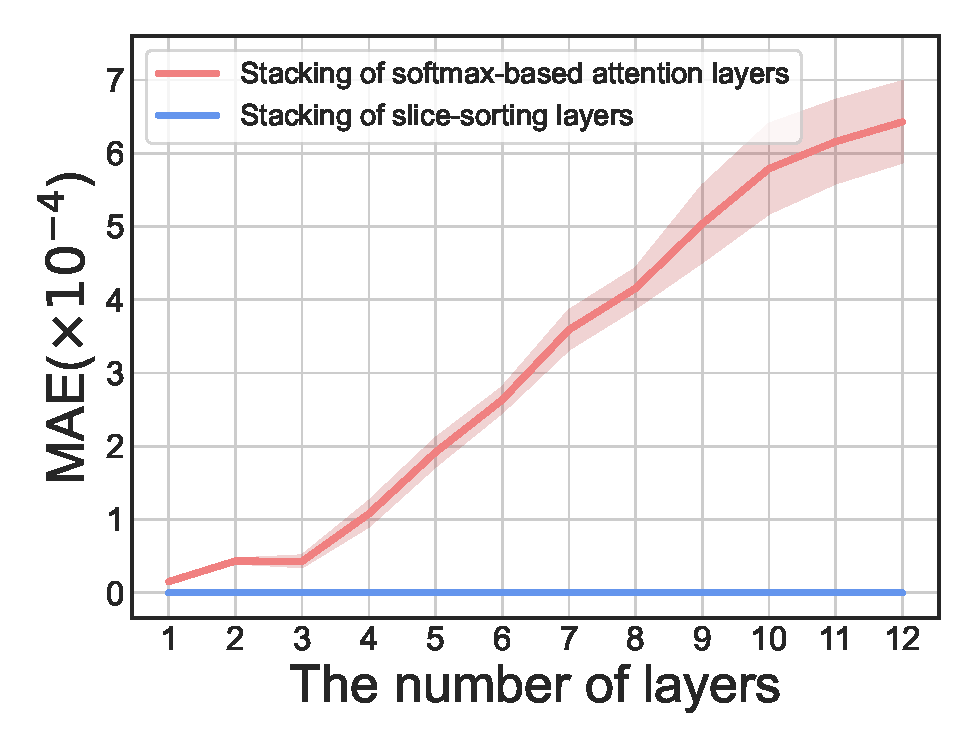
\includegraphics[height=4.3cm]{figures/MAE.pdf}\label{fig:cos}
  }
  \subfigure[Convergence of training process]{
  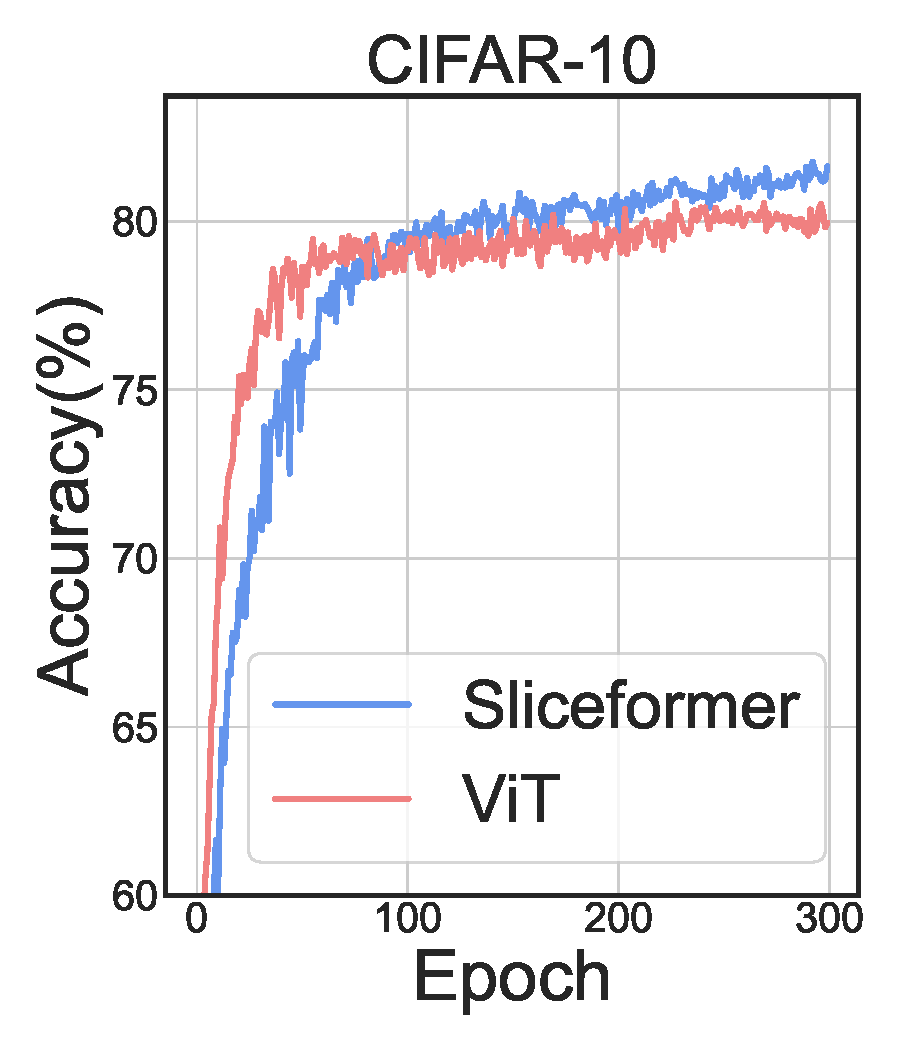
\includegraphics[height=4.5cm]{figures/converge_cifar10.pdf}\label{fig:convergence}
  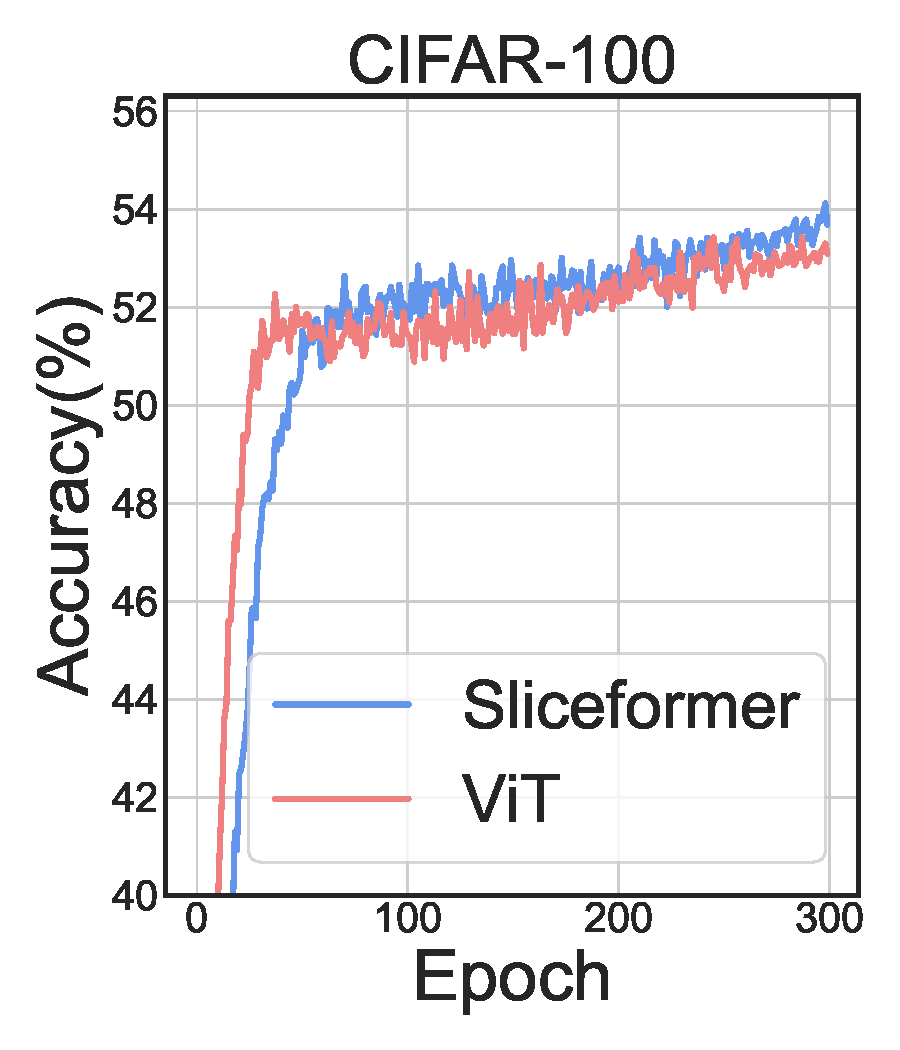
\includegraphics[height=4.5cm]{figures/converge_cifar100.pdf}\label{fig:convergence}
  }
  \caption{
  (a) The impact of the order of pixel sequence on the numerical permutation-invariance of model.
  (b) The comparison for our Sliceformer and ViT on their convergence when training on the CIFAR-10 and CIFAR-100 dataset.
  }
\end{figure}

\textbf{Molecular Analysis.}
Besides achieving a vision Sliceformer, we introduce the slicing-sorting operation to Graphormer~\cite{ying2021transformers} and test its impacts on molecular property prediction. 
In particular, the attention head of Graphormer applies a modified ``query-key-value'' architecture, which is formulated as $\text{Softmax}(\bm{S}+\bm{E}+\frac{1}{\sqrt{D}}\bm{QK}^{\top})\bm{V}$. 
Here $\bm{S}$ and $\bm{E}$ are learnable embedding matrices encoding spatial positions and edge information, respectively. 
% Applying the slicing-sorting operation, we design a simplified attention layer as $\text{Sort}_{\text{col}}(\text{Softmax}(\bm{S}+\bm{E})\bm{V})$, where the query and key matrices are ignored. 
Applying the slicing-sorting operation, we design a simplified attention layer without the query and key matrices and dramatically reduce the trainable parameters by around 30\%.
Replacing the attention layer of Graphormer with this layer leads to a Sliceformer for molecular data.
We apply the PCQM4M-LSC dataset~\cite{hu2021ogb} for training and testing the models. 
The experimental results in Table~\ref{tab:graphormer} show that applying the slicing-sort operation leads to a simplified model with a smaller size, whose performance is comparable to Graphormer.